\section{Results}

\subsection{The measurement gap is large in some years and spatially uneven}

MTA-reported availability and calendar continuity are close in some years and widely separated in others (Fig.~\ref{fig:trend}). The systemwide gap was 0.39 percentage points in 2018, 5.14 points in 2024, and 7.41 points in 2025. In 2025, MTA-reported availability was 97.61\%, while calendar continuity was 90.20\%. The 2026 values, covering January through October, were 97.25\% and 92.94\%, respectively.

\begin{figure}[htbp]
\centering
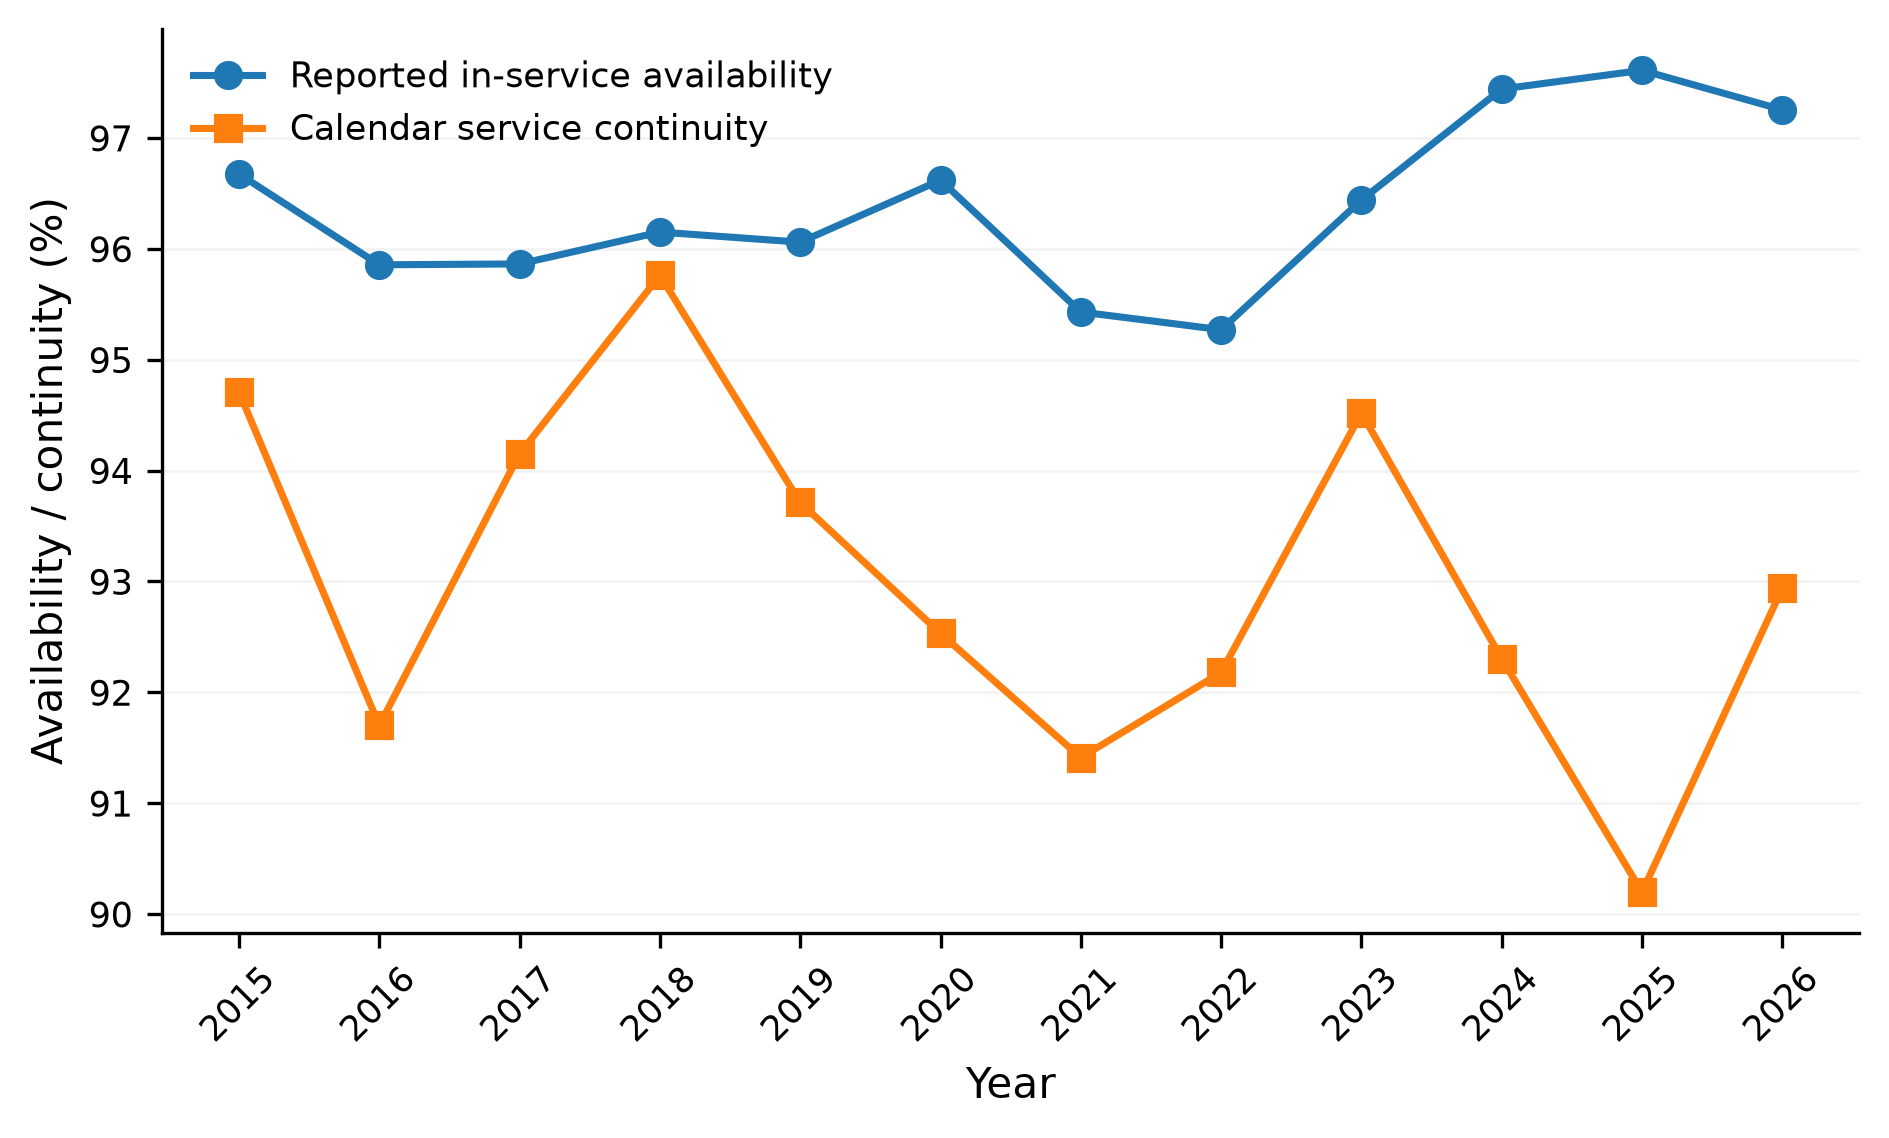
\includegraphics[width=0.92\linewidth]{fig2_metric_gap.png}
\caption{Annual MTA-reported elevator availability and calendar continuity, 2015--2026. The 2026 observation covers January--October. Annual values describe the asset composition observed in each year.}
\label{fig:trend}
\end{figure}

The 2025 gap also varied across boroughs (Table~\ref{tab:borough2025}). The Bronx combined 97.46\% MTA-reported availability with 81.70\% calendar continuity, producing a 15.77-point gap. Brooklyn and Queens also showed substantial differences, while Manhattan's gap was 5.20 points.

\begin{table}[htbp]
\centering
\caption{Borough-level elevator service measures, 2025.}
\label{tab:borough2025}
\begin{threeparttable}
\small
\begin{tabular}{lrrr}
\toprule
Borough & MTA-reported (\%) & Calendar (\%) & Gap (pp) \\
\midrule
Bronx & 97.46 & 81.70 & 15.77 \\
Brooklyn & 98.41 & 90.30 & 8.11 \\
Manhattan & 97.07 & 91.86 & 5.20 \\
Queens & 98.31 & 91.57 & 6.73 \\
\bottomrule
\end{tabular}
\begin{tablenotes}
\raggedright\footnotesize
\item The gap is MTA-reported availability minus calendar continuity.
\end{tablenotes}
\end{threeparttable}
\end{table}

The published metric is internally consistent. The difference arises because MTA-reported availability measures performance during time retained in the operator denominator, whereas calendar continuity retains the full calendar period.

\subsection{Denominator choice changes the geography of persistent low reliability}

Among the 113 station complexes with at least 36 observed months, seven fell in the lowest calendar-continuity quartile in at least half of their observed months. Figure~\ref{fig:map} maps those locations together with complexes showing a recurrence increase of at least 0.15 when calendar continuity replaces MTA-reported availability. These cut points are descriptive diagnostics rather than external service standards.

\begin{figure}[htbp]
\centering
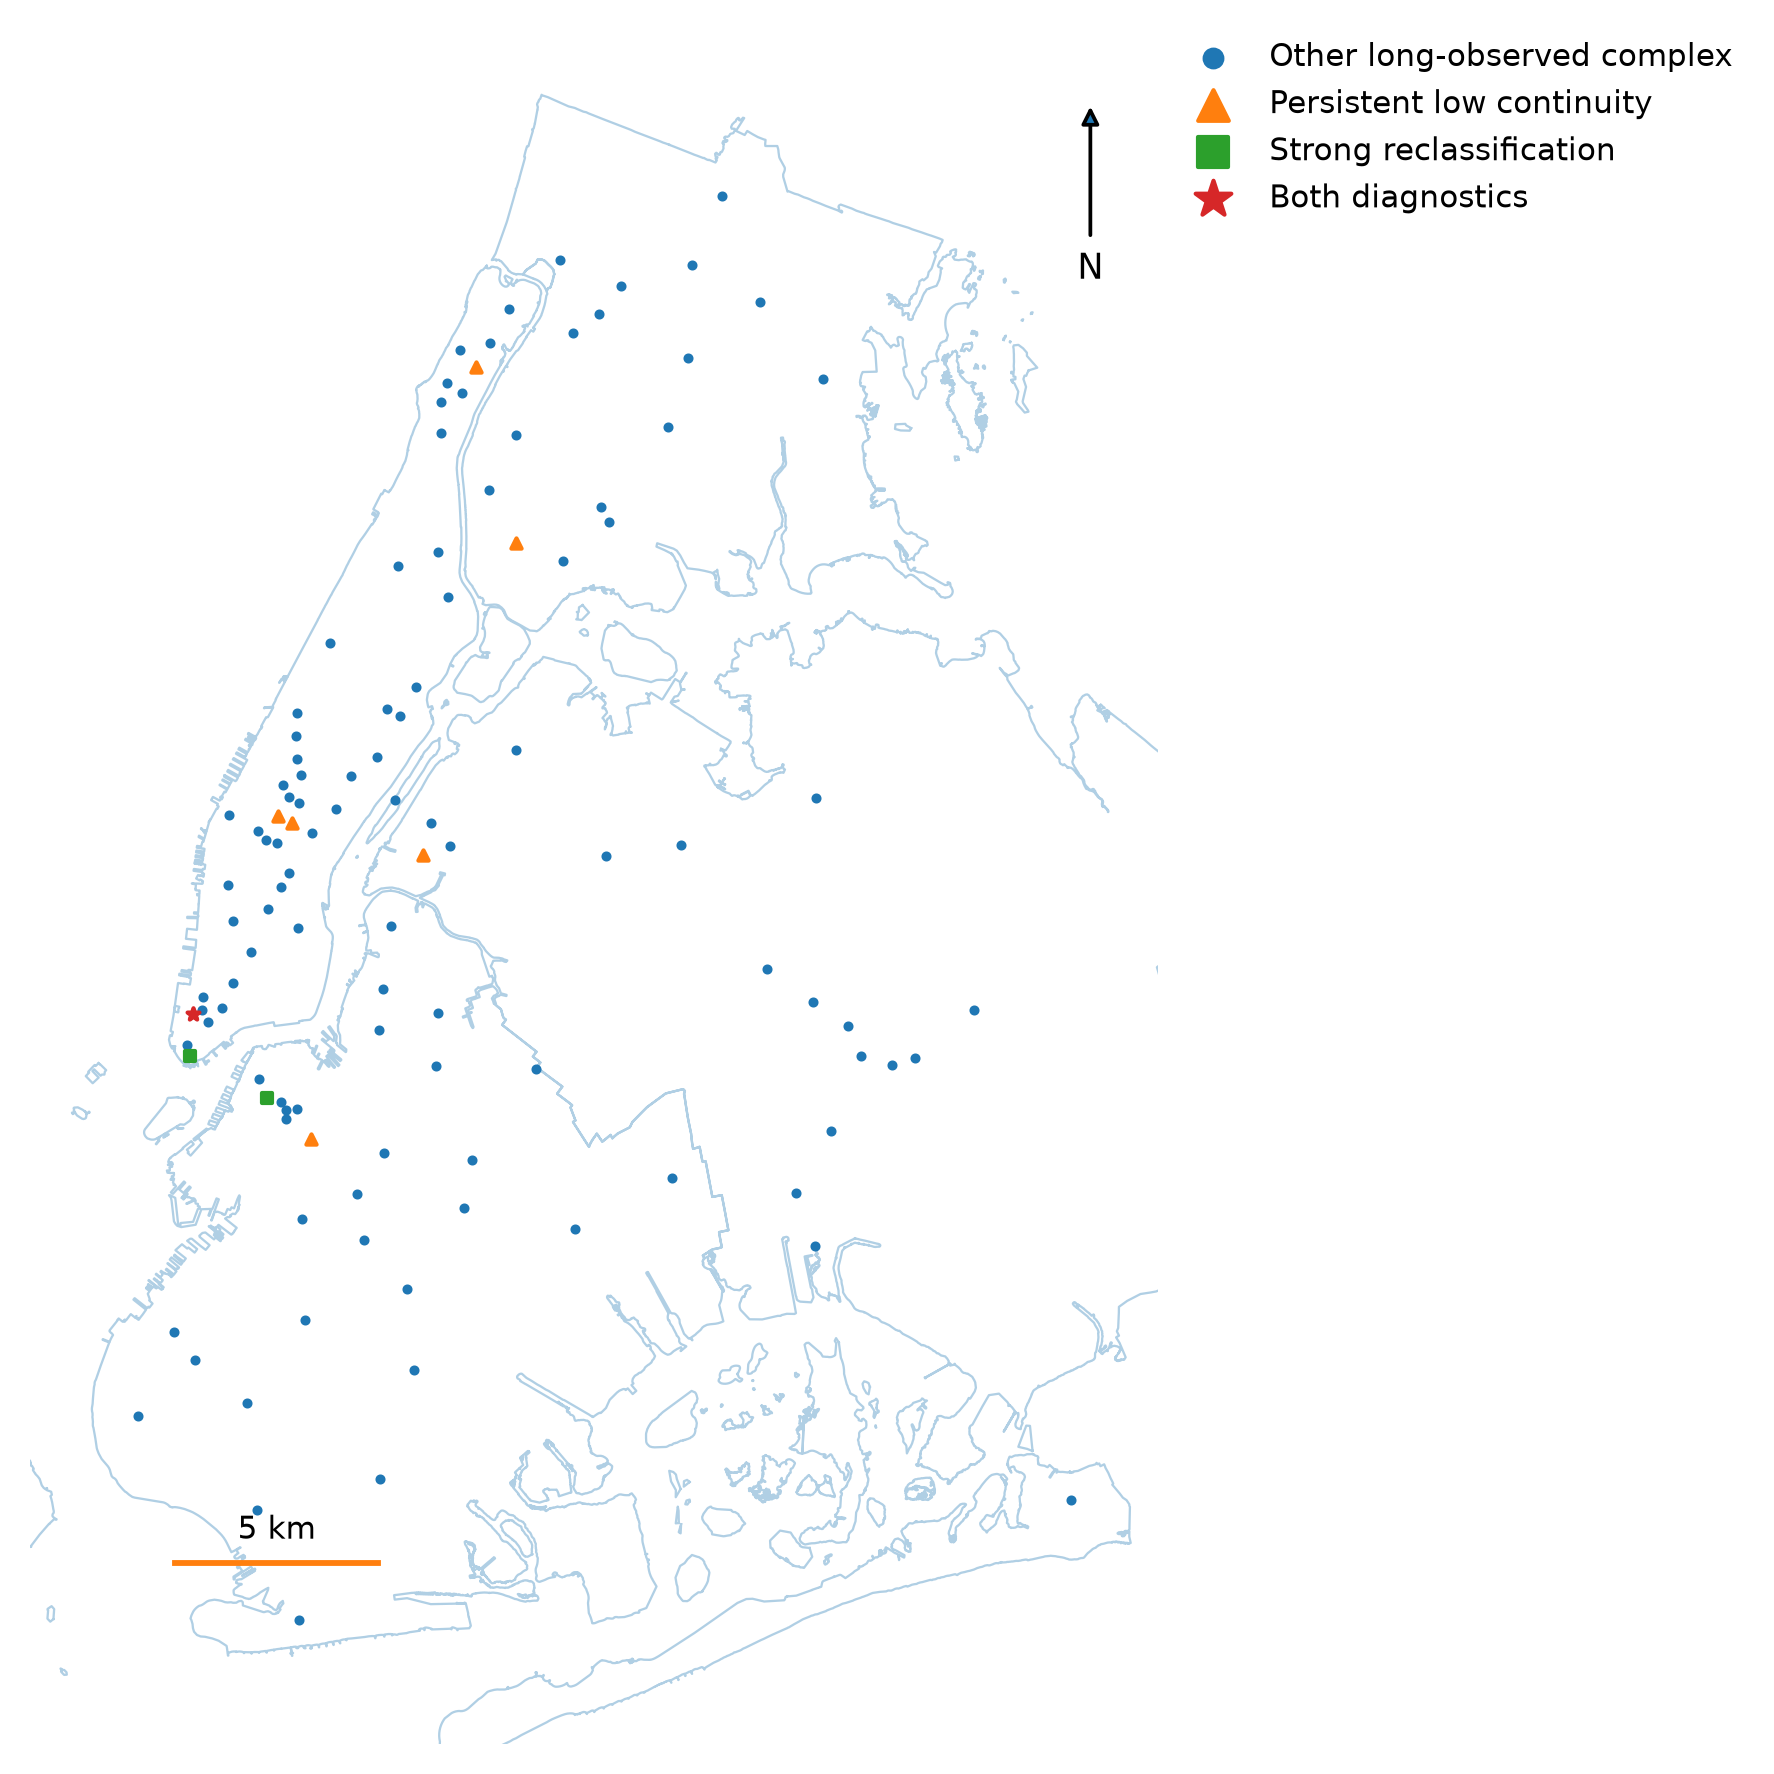
\includegraphics[width=0.88\linewidth]{fig1_spatial.png}
\caption{Spatial distribution of long-observed elevator-equipped station complexes. Symbols are mutually exclusive: persistent low continuity indicates membership in the lowest calendar-continuity quartile in at least 50\% of observed months; strong reclassification indicates an increase of at least 0.15 in low-reliability recurrence; both diagnostics indicates that both conditions are met. Station-complex coordinates are from MTA Subway Stations and Complexes, and borough boundaries are from the New York City Department of City Planning \citep{mta_stations2026,nycdcp_boroughs2026}.}
\label{fig:map}
\end{figure}

The largest reclassification occurred at Cortlandt Street (complex 328). It was in the monthly low-reliability quartile in 13.3\% of valid months under MTA-reported availability and 67.3\% under calendar continuity. South Ferry/Whitehall Street increased from 12.4\% to 29.6\%, while Court Street/Borough Hall increased from 26.1\% to 43.0\%. Figure~\ref{fig:reclass} shows the continuous recurrence difference across all eligible complexes.

\begin{figure}[htbp]
\centering
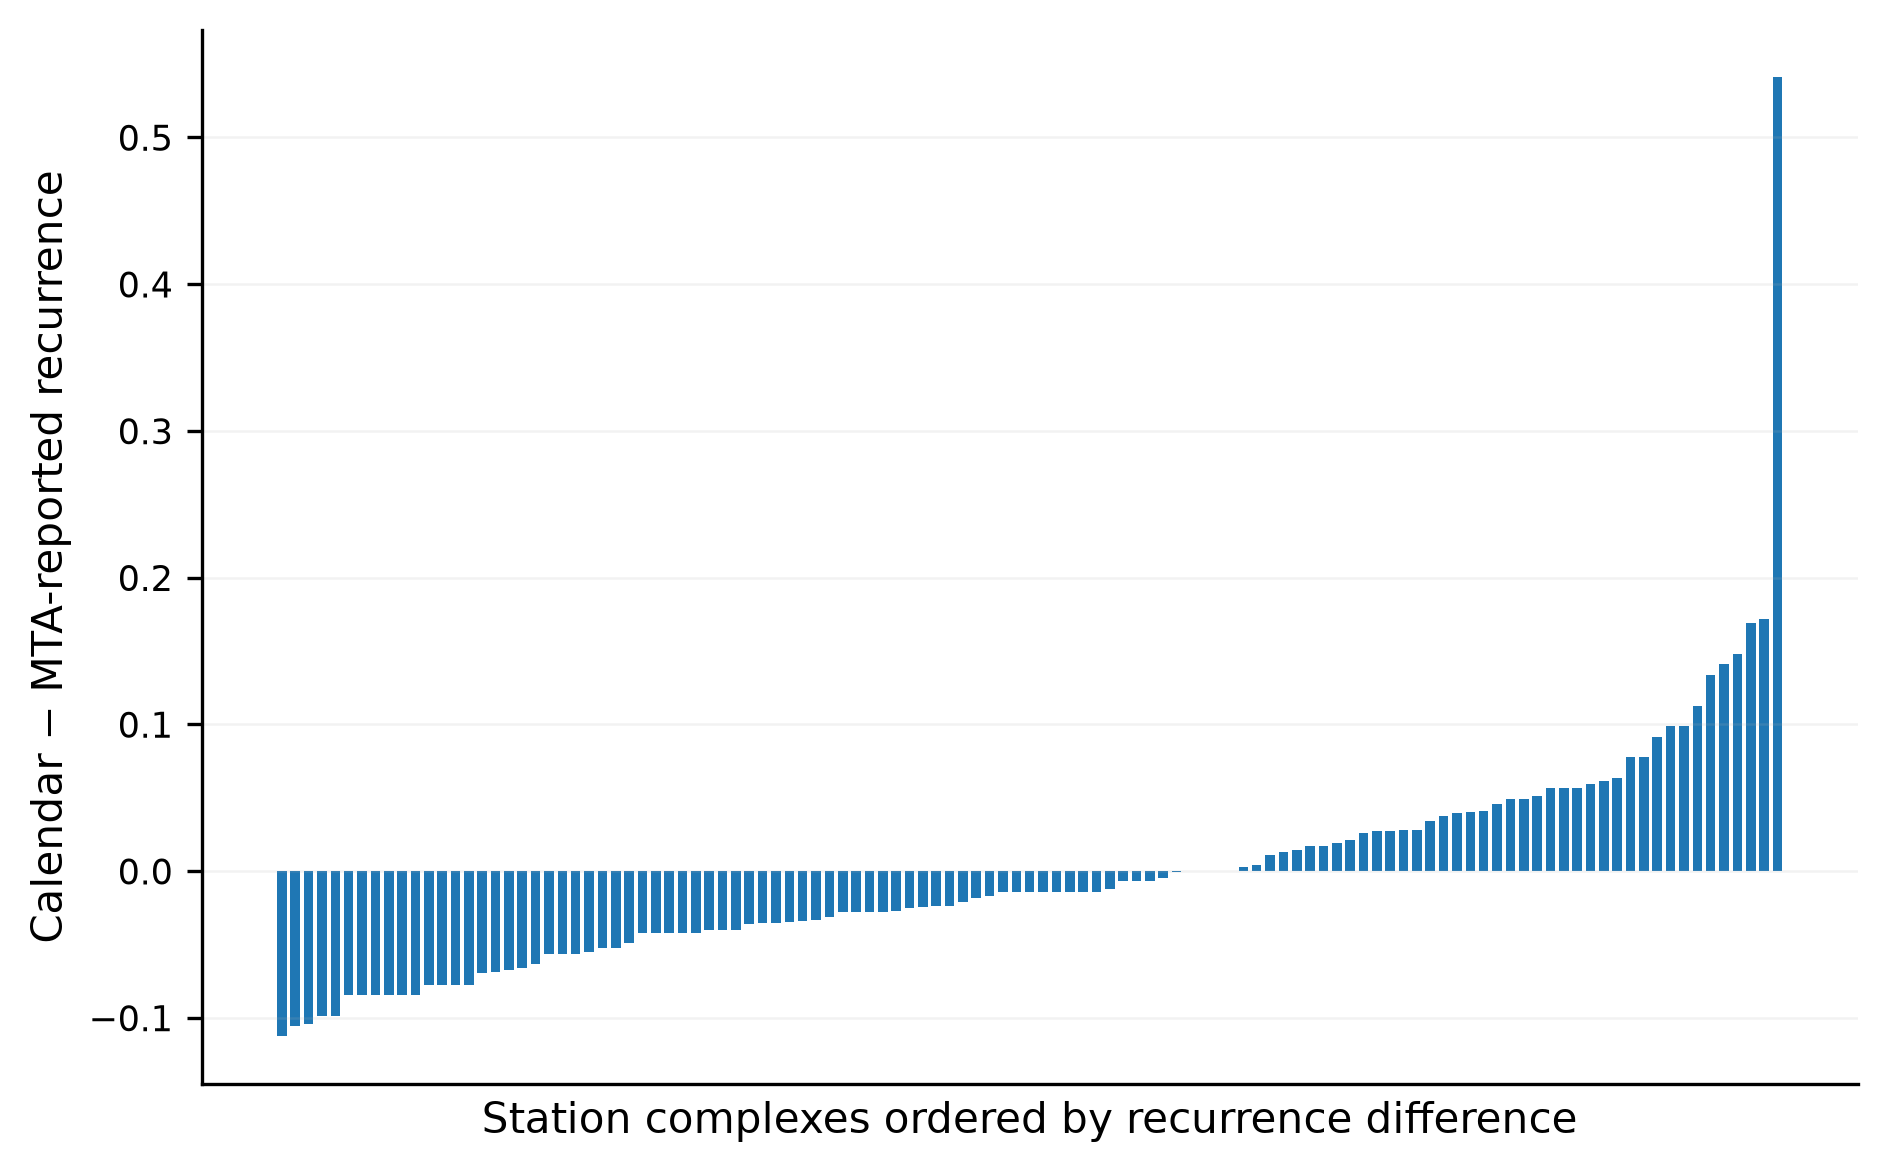
\includegraphics[width=0.72\linewidth]{fig3_reclassification.png}
\caption{Difference in station-complex low-reliability recurrence between calendar continuity and MTA-reported availability. Complexes are ordered by the recurrence difference. Positive bars indicate more frequent low-reliability classification when denominator-excluded calendar time is retained. Missing MTA-reported values are excluded from the corresponding recurrence denominator.}
\label{fig:reclass}
\end{figure}

The two recurrence measures remain strongly associated, but the relationship is not one-to-one. Under the primary 36-month and bottom-quartile specification, their Spearman correlation is 0.877. The three strongest reclassified complexes remain above the 0.15 recurrence-difference threshold when the low-reliability definition is changed to either the bottom quintile or the bottom tercile.

\subsection{Relative reliability is persistent under both service measures}

Station-complex rankings show substantial persistence from one year to the next. For MTA-reported availability, all eleven adjacent-year Spearman correlations are positive and statistically significant (Fig.~\ref{fig:persistence}). The mean is 0.562, with values from 0.405 in 2019--2020 to 0.666 in 2024--2025. Calendar continuity produces the same general pattern: the mean adjacent-year correlation is 0.525, with all eleven correlations positive and statistically significant.

\begin{figure}[htbp]
\centering
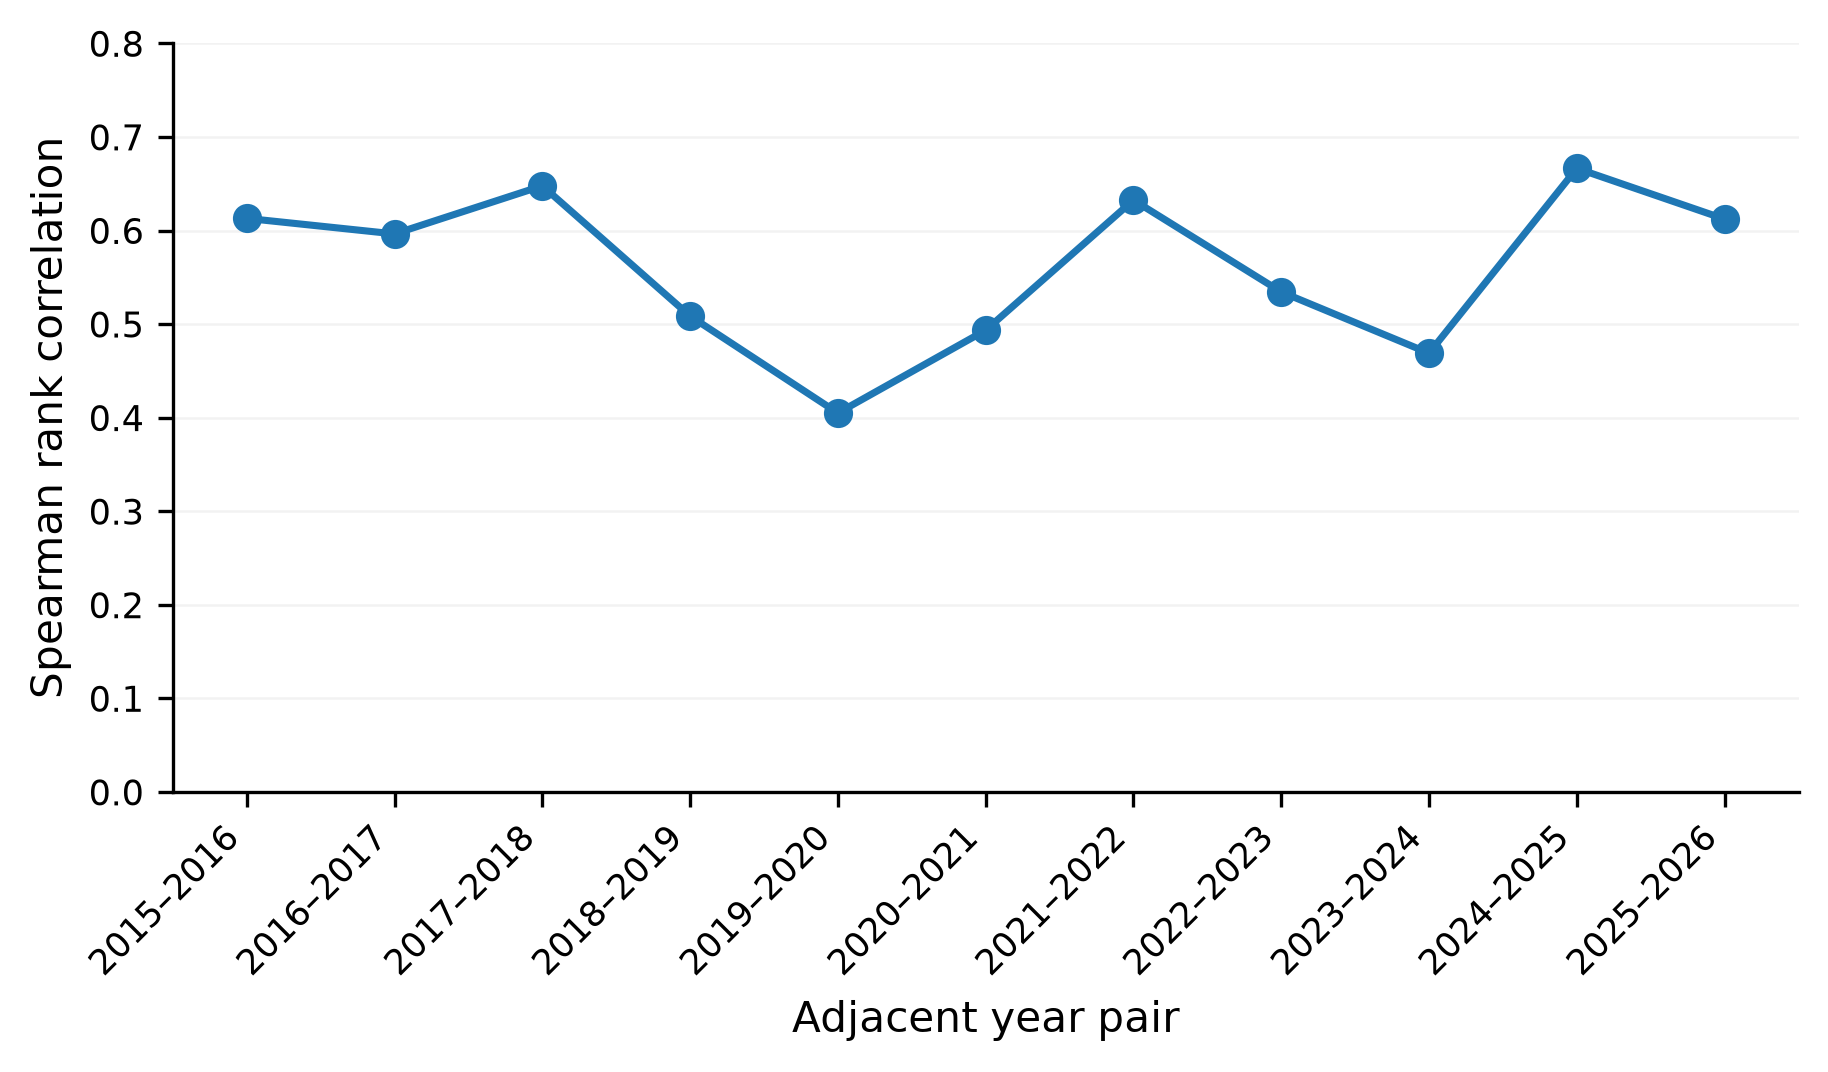
\includegraphics[width=0.92\linewidth]{fig4_persistence.png}
\caption{Spearman rank correlation of station-complex MTA-reported availability in adjacent years. Complexes must have at least six observed months in each year. The 2025--2026 pair uses January--October 2026; partial-year sensitivity results are reported in the text.}
\label{fig:persistence}
\end{figure}

The partial 2026 period does not drive the reported-availability result. Excluding the 2025--2026 pair changes the mean adjacent-year correlation from 0.562 to 0.557. When every year is restricted to January--October, the 2025--2026 correlation is 0.561 for MTA-reported availability and 0.477 for calendar continuity. Calendar-continuity persistence is shown separately in the Supplementary Material.

\subsection{Asset and platform metrics are related but spatially non-equivalent}

Across 420 borough--month observations in the overlapping 2018--2026 period, aggregated elevator MTA-reported availability and accessible-platform availability have a Spearman correlation of 0.697 and a mean absolute difference of 1.23 percentage points. Numerical association does not translate into stable spatial ordering. The complete four-borough ranking is identical in 11 of 105 complete months (10.5\%), and 64.5\% of borough rank positions change between the two measures.

Figure~\ref{fig:comparison} shows the month-by-month Kendall concordance of the four-borough rankings. The mean Kendall coefficient is 0.286, indicating that agreement in relative borough order varies substantially through time.

\begin{figure}[htbp]
\centering
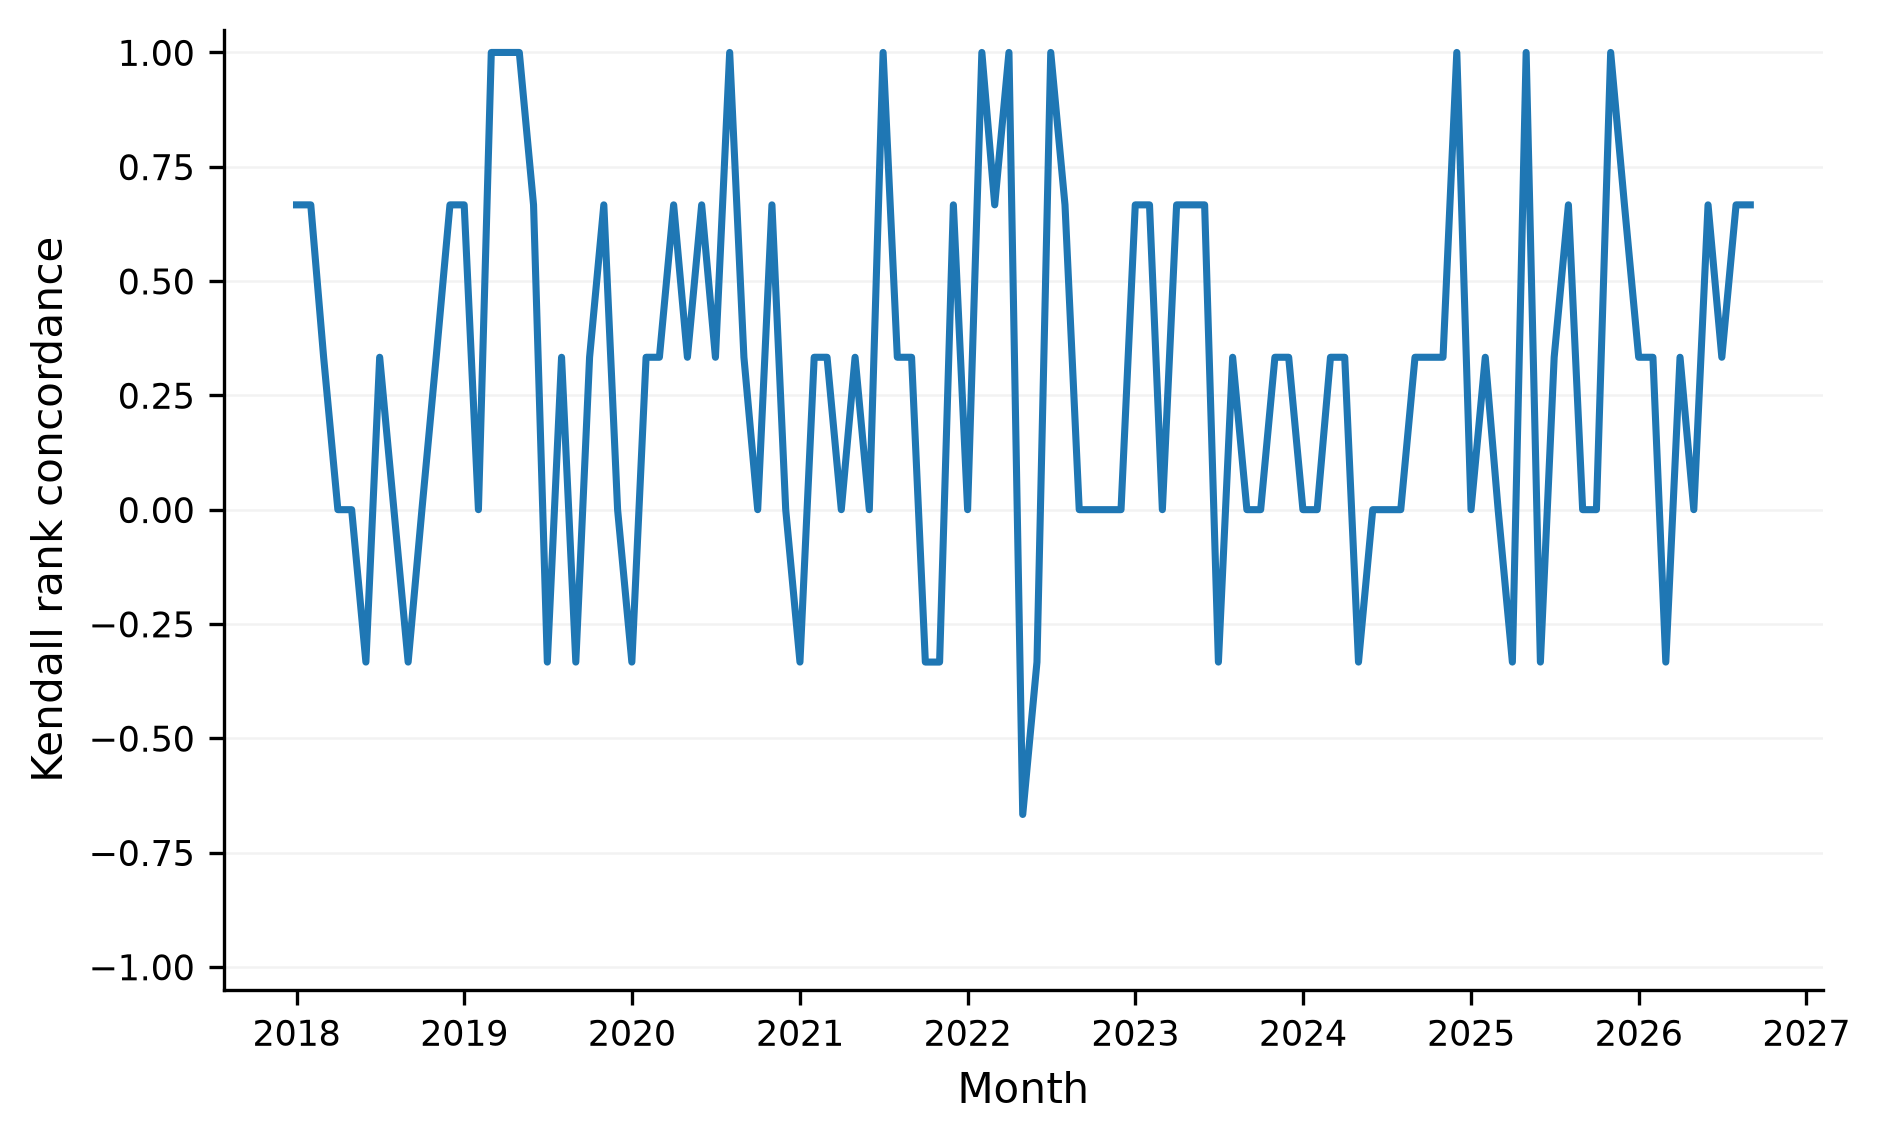
\includegraphics[width=0.92\linewidth]{fig5_concordance.png}
\caption{Monthly Kendall rank concordance between borough rankings derived from aggregated elevator MTA-reported availability and MTA accessible-platform availability, 2018--2026. A value of 1 indicates identical borough ordering.}
\label{fig:comparison}
\end{figure}

The two indicators operate at different spatial and functional levels. The comparison therefore shows concordance rather than validation: asset reliability and accessible-platform availability are related, yet they frequently prioritise boroughs differently.

\subsection{Sensitivity analyses support the measurement interpretation}

The 2025 calendar-time decomposition clarifies the source of the headline gap. Across all elevator records, 90.20\% of calendar hours were recorded as available. A further 2.21\% were unavailable within the MTA-reported denominator, while 7.59\% were excluded from that denominator. Excluded time therefore accounted for 77.5\% of total calendar service loss in 2025.

The borough pattern was concentrated rather than uniform within each borough. In the Bronx, excluded time represented 88.4\% of total calendar service loss, but 96.9\% of Bronx excluded hours came from the three station complexes with the largest excluded-hour totals. The single largest complex accounted for 63.3\%. The large Bronx gap should therefore be read as a borough-level concentration of specific station-complex conditions rather than a uniform borough-wide service state.

Removing the first and last observed month of every elevator changed 2025 systemwide calendar continuity from 90.20\% to 90.29\%. The longitudinal-coverage sensitivity is similarly stable. When the minimum observation requirement is varied from 24 to 72 months, the Spearman association between the two chronicity measures ranges from 0.863 to 0.877; seven complexes remain below the calendar-continuity quartile in at least half of their observed months, and three retain recurrence increases of at least 0.15.

Changing the descriptive low-reliability cut point also preserves the main reclassification pattern. Across bottom-quintile, quartile, and tercile definitions, the correlation between MTA-reported and calendar-continuity recurrence ranges from 0.814 to 0.906. Cortlandt Street, South Ferry/Whitehall Street, and Court Street/Borough Hall exceed a 0.15 recurrence increase under all three definitions.

Network expansion does not account for the measurement gap. A common-asset sensitivity panel contains 260 elevators observed for at least ten months in every year from 2015 through 2025. In that stable panel, the 2025 gap is 10.99 percentage points, compared with 7.41 points in the full 2025 system. The annual series in Fig.~\ref{fig:trend} is therefore descriptive of each year's system composition, while the denominator effect remains substantial under a fixed asset set.
